\section{Model Description}
\label{app:model_description}

In this section we sketch the process of moving from a real world scenario, to a minimal game which sufficiently captures reality. For a

Typically in the UK, a women will have 12 appointments with a midwife during the antenatal period, and in the majority of cases will encounter several different midwives \citep{Redshaw2014} in the course of their care. In the UK, and unlike most healthcare scenarios, maternity notes are held by the patient, so midwives do not have extensive information prior to an appointment unless they have encountered the woman previously. Maternity notes are not generally linked to extra-departmental records, meaning that a history of alcohol related admissions to another service may remain unknown unless revealed by the woman.

According to NICE guidance \citep{NICE2010a,NICE2010} the issue of substance misuse should be raised at the initial booking appointment, followed by subsequent action if a concern is raised is at the discretion of the midwife. This may take the form of specific guidance to reduce intake, or if deemed necessary a referral to a specialist midwife and relevant interdisciplinary team. On alcohol consumption, policy regarding how to determine the level of consumption is at the time of writing generally at the level of local health authority, hospital trust, or according to the best judgement of the individual midwife, with no guidance provided by NICE. This commonly takes the form of average units per week, but may include \ac{T-ACE}\footnote{The \ac{T-ACE} is a four question screening test for alcohol misuse intended specifically for use with pregnant women.} \citep{Sokol1989863} and similar measures. 

Beyond the \enquote{booking} appointment, the onus is on women to raise concerns about their drinking behaviour, or the midwife to probe further if they feel it is warranted. In either case, once a concern has been raised the midwife must respond clinically, and inevitably personally, to the information.

In an ideal world, all interactions with healthcare providers would be immediately and fully disclosive, with no repercussions for the patient. However, alcohol misuse by women is known to attract stigma \citep{Gomberg1988}, and is a recognised barrier to appropriate treatment in the maternity context \citep{NICE2010,Radcliffe2011}.

\subsection{Disclosure Game}
\label{sub:the_game}
%Outline how the scenario translates into a game.
%Brief mention of the game theoretic solution

In order to translate the scenario sketched above into a more abstract, tractable form, we cast it as a signalling game, and assume that women's disclosures (or not), are signals. We also make the simplifying assumption that a woman may have one of only three drinking patterns - light\footnote{Or abstinent, the extent of alcohol consumption being such that it would generally be felt to pose essentially no risk.}, moderate, or heavy. Correspondingly, they are limited in what signals they may send when claiming to be one of these three types. 

Midwives are treated in a similar fashion, where their type corresponds to how negatively they regard a drinking pattern - non-judgemental, moderately judgemental, and harshly judgemental. The expression of this judgement is not a matter of choice on their part, and is assumed to have no impact on their clinical response, which is to either refer the woman for specialist treatment, or do nothing.

At the end of a game, each player receives a payoff dependent on the actions and types of both players. Because both women and midwives have an interest in the outcome of the pregnancy, and would prefer a healthy baby, the payoff has a common interest component. Hence, both players receive a payoff based on the outcome of pregnancy, but women bear a social cost dependent on the signal they sent and the midwife's reaction to it. Similarly, midwives pay a cost if they refer to a specialist, mirroring the organisational cost of non-routine care. Table \ref{tab:Payoff-matrix} shows the three payoff matrices which together describe the game.

\begin{table}
\center
\subfloat[Social cost, \(X_{s}\), for women, given their signal, and the midwife's type\label{tab:Social-cost-matrix}]{%
\begin{tabular}{|c|c|c|c|c|}
\cline{3-5} 
\multicolumn{2}{c}{} & \multicolumn{3}{|c|}{Woman}\tabularnewline

\hline
\multirow{4}{*}{\rotatebox[origin=c]{90}{Midwife}} &  & Heavy & Moderate & Light\tabularnewline
\cline{2-5} 
 & Harsh & -2 & -1 & 0\tabularnewline
\cline{2-5} 
 & Moderate & -1 & 0 & 0\tabularnewline
\cline{2-5} 
 & Non & 0 & 0 & 0\tabularnewline
\hline 
\end{tabular}

}

\subfloat[Health outcome, \(X_{h}\), for women and midwives, given the midwife's action, and woman's type\label{tab:Referral-payoff-matrix}]{%
\begin{tabular}{|c|c|c|c|c|}
\cline{3-5} 
\multicolumn{2}{c}{} & \multicolumn{3}{|c|}{Woman}\tabularnewline

\hline 
\multirow{3}{*}{\rotatebox[origin=c]{90}{Midwife}} &  & Heavy & Moderate & Light\tabularnewline
\cline{2-5} 
 & Refer & 10 & 10 & 10\tabularnewline
\cline{2-5} 
 & Don't refer & -2 & -1 & 10\tabularnewline
\hline 
\end{tabular}

}

\subfloat[Referral cost, \(X_{c}\), for midwife, given their action and the woman's type\label{tab:inst_cost_matrix}]{%
\begin{tabular}{|c|c|c|c|c|}
\cline{3-5}  
\multicolumn{2}{c}{} & \multicolumn{3}{|c|}{Woman}\tabularnewline
\hline 
\multirow{3}{*}{\rotatebox[origin=c]{90}{Midwife}} &  & Heavy & Moderate & Light\tabularnewline
\cline{2-5} 
 & Refer & -9 & -9 & -9 \tabularnewline
\cline{2-5} 
 & Don't refer & 0 & 0 & 0\tabularnewline
\hline 
\end{tabular}

}

\caption{Payoff matrices\label{tab:Payoff-matrix}}
\end{table}

Taken together, this leads to a game tree that is relatively complex (figure \ref{fig:simple_tree} shows a simplified representation, with a detailed view of one branch in figure \ref{fig:zoom_tree}) even at the subgame level. 

As an example, consider the challenge faced by an agent of the heavy drinking type. In order to get the best health outcome, they must be referred and would ideally achieve this without paying any social cost at all. The best move depends on the type, and beliefs of the midwife. For example, a particularly unlucky scenario might be for the midwife to not only be of a harshly judgemental disposition, but to believe that no women really need to be referred. Even a relatively weak belief in this possibility can make the honest signal look like an unwarranted risk.

Rather than attempt to solve for equilibria, agents treat this two player game as taking place against nature, along the lines of adversarial risk analysis \citep{RiosInsua2009}. This effectively translates the game to a pair of decision problems (figure \ref{fig:decision_problems}), which agents attempt to resolve at each turn using a simple decision rule, given their prior beliefs and experience of play.

\begin{figure}[H]
\begin{adjustbox}{center}
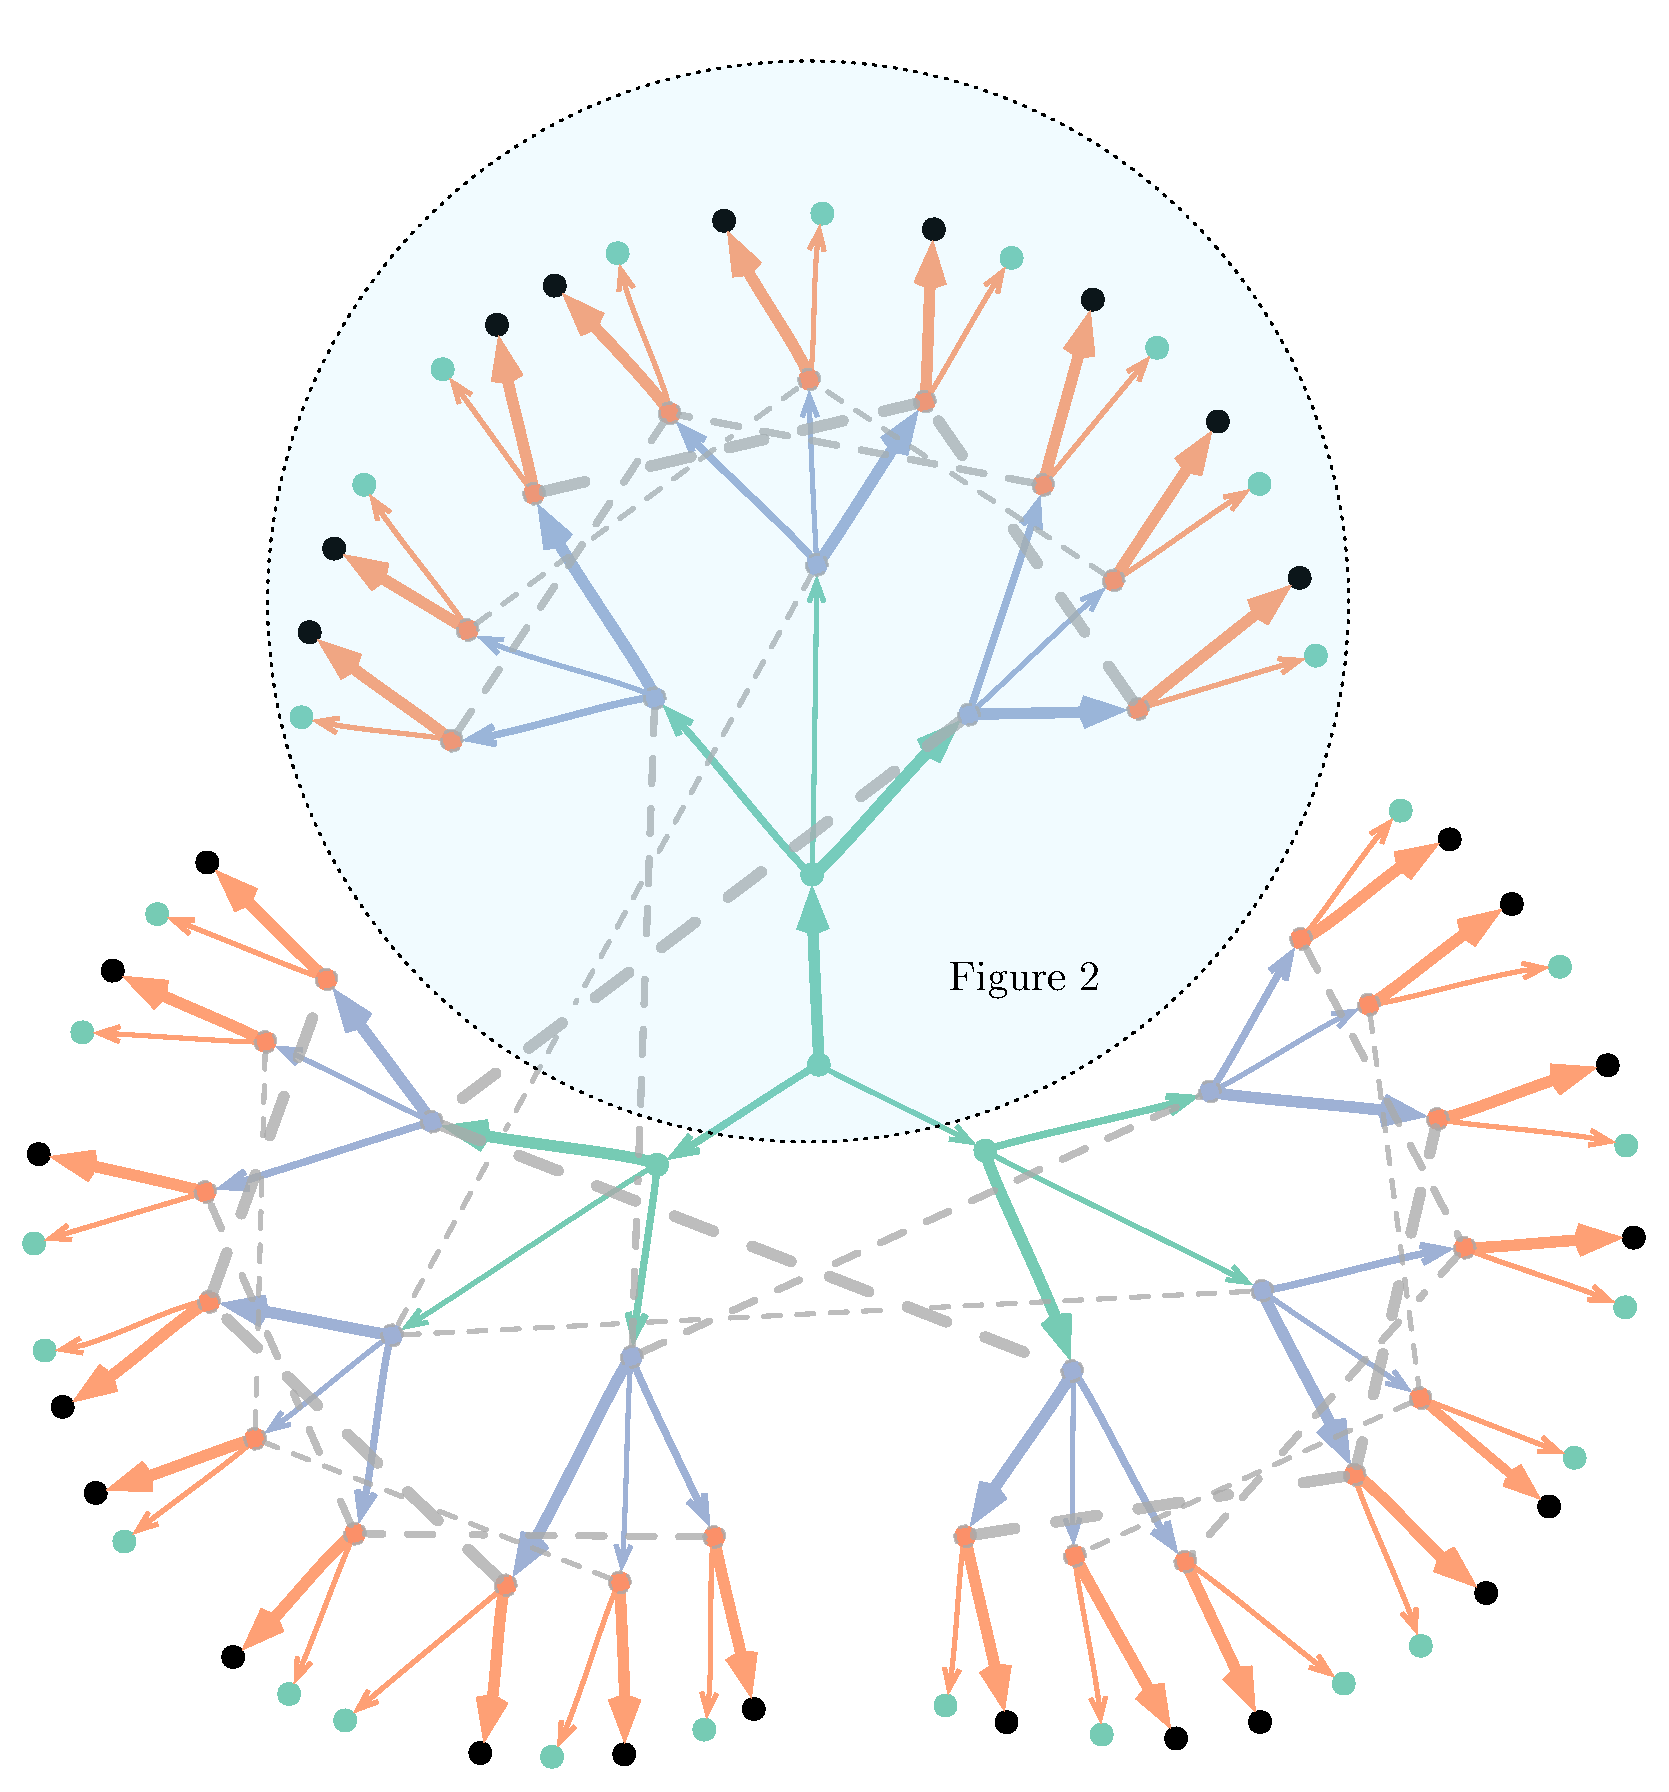
\includegraphics[width=119mm]{figures/rounded_clover_infosets}
\end{adjustbox}
\caption{Simplified game tree. Arrows correspond to two moves by nature, followed by women, and midwives respectively. Line weight distinguishes between information sets, and possible moves, corresponding to ascending player types. For midwives, referral is shown by a heavier arrow. Light terminal nodes indicate that the game may repeat from that point, and black nodes are exits}

\label{fig:simple_tree}
\end{figure}

\begin{figure}[H]
\begin{adjustbox}{center}
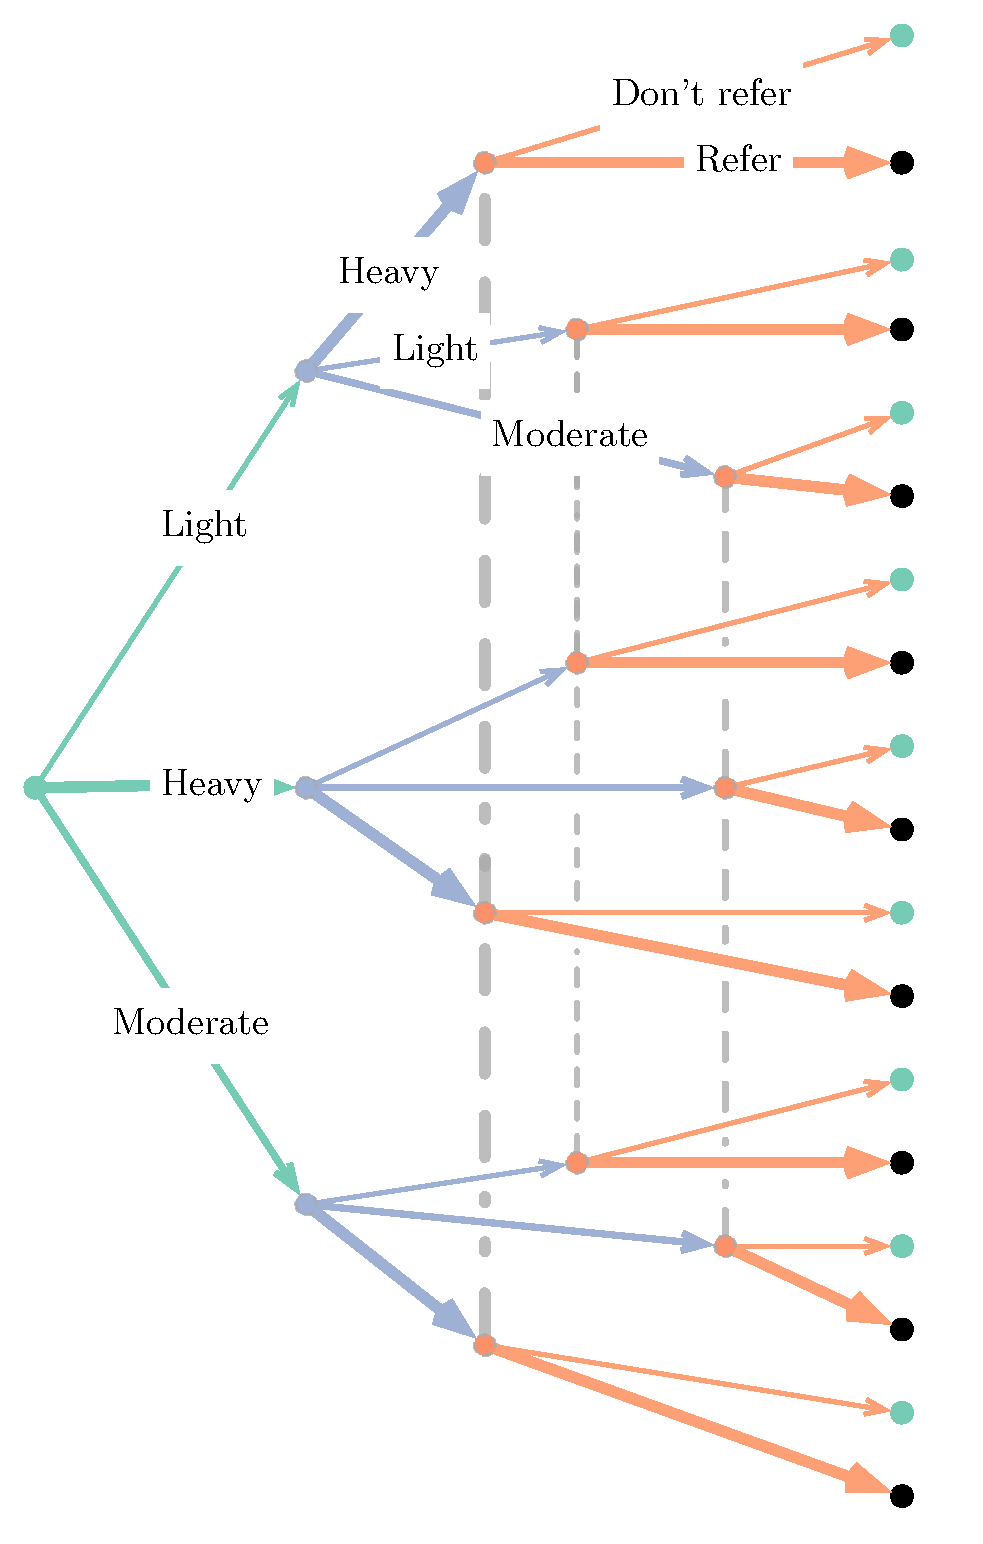
\includegraphics[width=119mm]{figures/tree_zoom}
\end{adjustbox}
\caption{Detail view of a single game tree branch, showing the possible moves by each player, with information sets for midwives}

\label{fig:zoom_tree}
\end{figure}

\begin{figure}[H]
\begin{adjustbox}{center}\subfloat[Women (heavy drinkers)]{\includegraphics[width=119mm]{figures/women_influence}}\end{adjustbox}
\vskip
\begin{adjustbox}{center}\subfloat[Midwives]{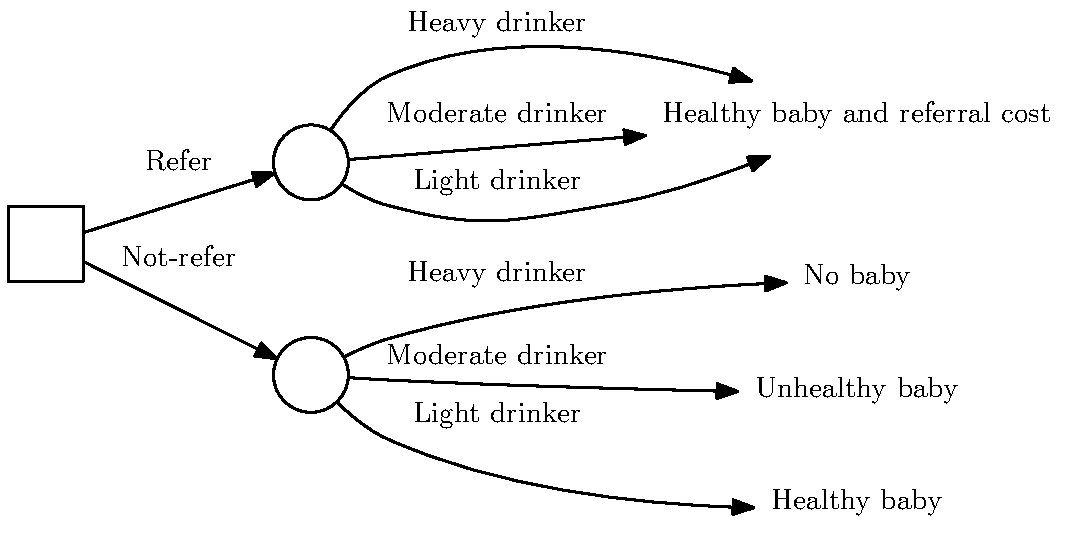
\includegraphics[width=119mm]{figures/mw_influence}}\end{adjustbox}
\caption{Influence diagrams, showing the game broken into two decision problems. Squares indicate a decision node, while circles are (from the perspective of the agent) chance nodes}

\label{fig:decision_problems}
\end{figure}

%Might belong in a more methody bit? Read some stuff to check..
To formally define the game, let \(N = \{m, w\}\) be the set of players each with a private type \(\theta_{i} \in \Theta\), and a set of types \(\Theta=\{l, m, h\}\), with pure strategies \(A_{m}=\{r,n\}, A_{w}=\{l, m, h\}\). Here, \(\{l, m, h\}\) correspond to light, moderate, and heavy alcohol consumption for women, and non-judgemental, moderately judgemental, and harshly judgemental for midwives. Midwives' pure strategies \(\{r,n\}\) are to refer, or do nothing, and those for women are to signal that they have one of the possible drinking patterns.
Additionally define two utility functions - 
\begin{equation}
u_{w}(s_{w}, s_{m}, \theta_{w}, \theta_{m})=X_{s, s_{w}, \theta_{m}} + X_{h, \theta_{w}, s_{m}}
\end{equation} 
\begin{equation}
u_{m}(s_{w}, s_{m}, \theta_{w})=X_{h, \theta_{w}, s_{m}} + X_{c, \theta_{w}, s_{m}},
\end{equation} with $X_{c}$, $X_{h}$, and $X_{s}$ being the payoff matrices as in table \ref{tab:Payoff-matrix}, $s_{w}$ and $s_{m}$ denoting a specific signal by a woman, and referral response by a midwife. Lastly let \(p_{w}(l, m, h)\), \(p_{m}(l, m, h)\) be distributions over types of women, and midwives respectively.


As noted, rather than solve the game, we allow populations of agents to play it, and hence stipulate further that women are drawn in order from a queue of \(n_{w}\) women (where \(n_{w}=1000\) in all simulations), and play against a midwife chosen at random from a population of \(n_{m}\) (\(n_{m}=100\)). They play for a maximum of \(r_{w}\) rounds (\(r_{w}=12\) following the routine number of ante-natal appointments in the UK \citep{NICE2010a}) or until they are referred, and a new player is drawn from the same distribution that produced the original players to replace them. If they are not referred, they rejoin the back of the queue after their appointment. In either case, they are informed of their payoff after each round and update their beliefs accordingly using one of the rules described in section \ref{sub:the_agents}.

Midwives play for \(r_{m}\) rounds (\(r_{m}=1000\) in all experiments), and conduct appointments in parallel, i.e. if there are 5 midwives, then five women are drawn from the queue and assigned at random to the midwives. 
Unlike women, midwives are only informed of their payoff if they choose to make a referral. Both groups of agents have perfect recall, and midwives are assumed to retrospectively update their observations if they make a referral after a number of appointments.



\subsection{Agent Models}
\label{sub:the_agents}
%Outline basic structure, then specifics on each one.
%This should probably go lexic -> bayes payoff -> bayes -> CPT in order
% of complexity.
%suggest there are added shells of complexity
%		mention the info sharing because homophilly
%			related - the enhancement to the bayes/cpt agents is that they personalise, as much as anything.
%		properly explain dirichlet priors
% How about comparing the decision problem representation for the agent types?

While in principle a wide variety of agent models are possible, given that decision rules operate on essentially the same information, and produce the same outputs, we limit ourselves here to four. The simplest is a lexicographic rule (1), in the spirit of a \ac{FFH} \citep{Gigerenzer2004} which uses only information about payoffs given actions; this is followed by a Bayesian risk minimisation rule (2) using the same information; a second Bayesian risk rule (3) which uses information about the underlying lottery; and a two-stage \ac{CPT} \citep{Hau2008} agent (4) which is identical to 3, but uses the \ac{CPT} decision rule from \cite{Tversky1992}. Hence, each successive decision model adds a layer of sophistication to the problem representation while retaining the same input-output characteristics.

As noted in section \ref{sub:the_game}, agents have perfect recall, and midwives recognise women if they repeatedly encounter them. While agents recall perfectly and make use of the new information for retrospective updates, all four agent models make decisions `as-if' they were always facing a new \enquote{opponent}.

A simplifying assumption is made that all midwives have just qualified after receiving identical training. As a result, they have homogeneous beliefs about  women and assume to some extent that they are honest.
Women have heterogeneous beliefs, which correspond to experiencing \(k\) randomly chosen paths through the game, and following each path at least once.


\subsubsection{Lexicographic Heuristic}
\label{sub:lexico}

The lexicographic heuristic (algorithm \ref{alg:lexico}) follows the form of that used in \cite{Hau2008}, and assumes a simplified problem representation, where an action is a choice between combined lotteries. Functionally, the heuristic maintains a count of the number of times that each action was followed by a payoff, and chooses the action which most commonly has the best payoff, i.e. one reason decision making. Where there is no clear best action, but one or more is evidently worse, a choice must be made as to whether to discard the poorer action; in this case we have elected to retain it.
This approach requires minimal computation, and does not assume that \(u_{i}\) is static, or known.

Women resolve this by approximating the utility function, as a function \(f(s_{w}, \sigma)\) on their choice of signal and an unknown distribution $\sigma$, which maps to \(u_{w}\) - i.e. \(s_{w}\) is a choice between simple lotteries. The algorithm maintains a count, \(n\), of the number of occurrences of each outcome given the choice from \(s_{w}\).

Midwives solve a slightly different problem with more information, where \(s_{w}\) is known, and \(s_{m}\) is the lottery choice - \(f(s_{w}, s_{m},\sigma)\). This is resolved by maintaining a separate count for each signal (i.e. \(n_{s_{w},s_{m}}\)), and otherwise following the same algorithm, presented below.

\begin{algorithm}
\begin{algorithmic}
\State n=1, action=none
\While{action is none}
\State Calculate the nth most common outcome following each action.
\State Sort actions by the value of the nth most common outcome.
\If{clear winner} \State action = best \EndIf
\State n = n + 1
\EndWhile
\State \Return action
\end{algorithmic}
\caption{Lexicographic heuristic\label{alg:lexico}}
\end{algorithm}

As an example, take a light drinker who has played three rounds with a succession of particularly judgemental midwives, signalling honestly in two and claiming to be a moderate drinker in one. The most common outcome of the honest signal was a payoff of 10, which is clearly preferable to the 9 gained by claiming to be moderate. On that basis, they choose to signal honestly.

\subsubsection{Bayesian Payoff}

The Bayesian payoff agent uses the same subset of information as the lexicographic method, but updates beliefs on the link between actions and payoffs using the Bayes rule, and attempts to choose the action which minimises risk.

Given the discrete nature of actions and payoffs, coupled with a desire for tractability of the
simulation, the Dirichlet distribution is employed as a prior to represent these beliefs. The probability
density function takes the form -

\begin{equation}
D(\Theta|\alpha)=\frac{\Gamma(\sum_{i=1}^{k}\alpha_{i})}{\prod_{i=1}^{k}\Gamma(\alpha_{i})}\overset{k}{\underset{i=1}{\prod}\Theta_{i}^{\alpha_{i-1}}}
\end{equation}


where \(\alpha=\{\alpha_{1}\ldots\alpha_{k}\}\), \(k\) is the number
of signal-payoff pairs, \(\Theta=\{x_{1},\,\ldots,x_{k-\text{1}}\}\) all
more than zero and summing to less than 1, and \(\alpha_{i}\) is the 
pseudo-count of prior observations for a pair \(i\). 

The distribution is particularly convenient, in that to infer the
probability of a signal implying a payoff becomes
simply -

\begin{equation}
p(x=j|D,\alpha)=\frac{\alpha_{j}+n_{j}}{\sum_{j}(\alpha_{j}+n_{j})}\label{eq:posterior}
\end{equation}


Where \(n_{j}\) is simply the count of occurrences of signal-payoff pair \(j\), so
that the belief that a signal will lead to a payoff is the number
of times that pairing has been observed (including the pseudo-count),
over the total number of observations thus far. This makes computation
of beliefs fast and simple, since all that must be maintained is
a count of observations with no particular concern as to their order.
As before, midwives follow a similar pattern but maintain \(n_{s_{w}}\) independent counts of pairings between referral choice and payoff, updating their beliefs about the relationship between the choice to refer and payoff given the signal they have received.

Agents then choose the strategy $s_{i}$ to minimise risk $R_{i}$, which is simply defined as - 
\begin{equation}
R_{w}(s_{w}) = \sum_{x \in X} -xp(x | s_{w})
\end{equation}
\begin{equation}
R_{m}(s_{w}, s_{m}) = \sum_{x \in X} -xp(x | s_{w}\wedge s_{m}),
\end{equation}

where $X$ is the set of payoffs the agent has observed to follow $s_{i}$.


If we take our light drinker from the lexicographic case, and assume that they began with an uninformative prior. The 6 possible signal-payoffs pairings are then \([(l,10),(m,10),(h,10),(m,9),(h,9),(h,8)]\), with \(\alpha_{i}=1\) for all \(i\). After playing the three rounds, \(n_{l,10}=2\), and \(n_{m,9}=1\).

The agent then evaluates \(R_{w}\) for each signal, e.g. for the light signal:

\begin{equation*}
\begin{align*}
X &= \{10\}\\
R_{w}(l) &= \sum_{x \in X} -xp(x | l) = -10p(10 | l)\\
R_{w}(l) &= -10(\frac{\alpha_{l,10}+n_{l,10}}{\sum_{j}(\alpha_{j}+n_{j})}) = -10(\frac{1+2}{1+2})\\
R_{w}(l) &= -10(\frac{3}{3}) = -10
\end{align*}
\end{equation*}

and by the same method, \(R_{w}(m)=-9\frac{1}{3}\), and \(R_{w}(h)=-9\), concluding that signalling honestly is the best move.

\subsubsection{Bayesian Risk Minimisation}

The second Bayesian agent augments the reasoning of the simple payoff model, making the stronger assumption that the utility function is static, and known. Women maintain two sets of beliefs, corresponding respectively to \(p_{m}\), and the probability of referral given signal choice. This leads to the risk function, minimised with respect to \(s_{w}\) -

\begin{equation}
R_{w}(s_{w}, \theta_{w}) = \sum_{i\in A_{m}}\sum_{j\in \Theta} -u_{w}(s_{w}, i, \theta_{w}, j)p(j)p(i | s_{w}),
\end{equation}

so that the risk of a signal is the sum of the products of all payoffs with the probabilities of their entailed midwife types and responses.

Midwives reasoning centres on determining the meaning of signals, since given the knowledge of what some signal \(s_{w}\) conveys about the true type of the sender, the payoff for an action is known. As such, their inference process is the same as for the simple Bayesian agent but over signal-type pairs, and they attempt to minimise the following risk function, minimised with respect to \(s_{m}\) -

\begin{equation}
R_{m}(s_{w}, s_{m}) = \sum_{i\in \Theta} -u_{m}(s_{w}, s_{m}, i)p(i | s_{w})
\end{equation}

Returning to our example agent, under this model the type of the midwife becomes salient, hence \(n_{h}=3\), and \(n_{l,n}=2\), \(n_{m,n}=1\). Their prior beliefs remain uninformative, i.e. \(\alpha_{j} = 1, j \in \{l,m,h\}\), \(\alpha_{i,j}=1,i \in \{r,n\}, j \in \{l,m,h\}\). As before, the agent evaluates \(R_{w}\) for the three signals, and the process for the light signal is given below -

\begin{equation*}
\begin{align*}
R_{w}(l, l) &= \sum_{i\in A_{m}}\sum_{j\in \Theta} -u_{w}(l, i, l, j)p(j)p(i | l)\\
R_{w}(l, l) &= -u_{w}(l, r, l, l)p(l)p(r | l) - u_{w}(l, n, l, l)p(l)p(n | l) - u_{w}(l, r, l, m)p(m)p(r | l) - u_{w}(l, n, l, m)p(m)p(n | l) \\
&\phantom{{}=1}- u_{w}(l, r, l, h)p(h)p(r | l) - u_{w}(l, n, l, h)p(h)p(n | l)\\
u_{w}(l, i, l, j) &= 10\\
R_{w}(l, l) &= -10p(l)p(r | l) - 10p(l)p(n | l) - 10p(m)p(r | l) - 10p(m)p(n | l) - 10p(h)p(r | l) - 10p(h)p(n | l)\\
p(l) &= \frac{1 + 0}{1 + 1 + 1 + 3} = \frac{1}{6}\\
p(m) &= \frac{1 + 0}{1 + 1 + 1 + 3} = \frac{1}{6}\\
p(h) &= \frac{1 + 3}{1 + 1 + 1 + 3} = \frac{2}{3}\\
p(r | l) &= \frac{1 + 0}{1 + 1 + 2} = \frac{1}{4}\\
p(n | l) &= \frac{1 + 2}{1 + 1 + 2} = \frac{3}{4}\\
R_{w}(l, l) &= -10\cdot \frac{1}{6} \cdot \frac{1}{4} - 10\cdot \frac{1}{6} \cdot \frac{3}{4} - 10\cdot \frac{1}{6} \cdot \frac{1}{4} - 10\cdot \frac{1}{6} \cdot \frac{3}{4} - 10\cdot \frac{2}{3} \cdot \frac{1}{4} - 10\cdot \frac{2}{3} \cdot \frac{3}{4}\\
&= -10
\end{align*}
\end{equation*}

and similarly for moderate (\(R_{w}(m,l)=-9\frac{1}{3}\)), and heavy (\(R_{w}(h,l)=-8\frac{1}{2}\)) signals, once again concluding that honesty is the better option.

\subsubsection{Descriptive Decision Theory}

The most complex decision rule used is \ac{CPT}, which attempts to reproduce a number of systematic deviations from rationality observed in humans. While \ac{CPT} has primarily been applied in the context of decisions from description, it has been modified to deal with decisions from experience by incorporating a first stage where probabilities are estimates from observations as in \cite{FoxCPT}. In this instance the Bayesian inference process fills the first stage role.

%Maybe cut this bit and make explanation richer?
Rather than the psychologically more interesting \ac{PT}, the \ac{CPT}
decision rule is used in this instance, because of the requirement
for women to evaluate the `prospects'\footnote{Where a prospect is a sequence of payoff-probability pairings in ascending order of payoff, associated with an action.} of more than two actions. \ac{CPT} uses transformed probabilities, underweighting
small probabilities, and overweighting large ones. This is intended to reflect the observed behaviour of humans, where sufficiently high likelihoods are treated as certain, and contrastingly low probabilities as impossible. The correct weighting function is subject to some debate, but here we have used that of \citet{Tversky1992}, which treats probabilities differently for gains (eqn \ref{eqn:cpt_p_pos}) and losses (eqn \ref{eqn:cpt_p_neg}) -

\begin{align}
w^{+}(p) & = \frac{p^{\gamma}}{(p^{\gamma}+(1-p)^{\gamma})^{\frac{1}{\gamma}}}\label{eqn:cpt_p_pos}\\
w^{-}(p) & = \frac{p^{\delta}}{(p^{\delta}+(1-p)^{\delta})^{\frac{1}{\delta}}}\label{eqn:cpt_p_neg},
\end{align}


where $p$ is the unweighted probability, and $\gamma$ and $\delta$
are the weights for gain and loss probabilities respectively. Along similar lines, the values of losses and gains are transformed to reflect a tendency to regard a loss as more significant than a gain  -

\begin{equation}
v(u_{i})=\begin{cases}
f(u_{i}),& \text{if}\, u_{i}>0\\
0,& \text{if}\, u_{i}=0\\
\lambda g(u_{i}),& \text{if}\, x<0
\end{cases},
\end{equation}


where,

\begin{equation}
f(u_{i})=\begin{cases}
u_{i}^{\alpha},& \text{if}\,\alpha>0\\
\ln(u_{i}),& \text{if}\,\alpha=0\\
1-(1+u_{i})^{\alpha},& \text{if}\,\alpha<0
\end{cases}
\end{equation}
\begin{equation}
g(u_{i})=\begin{cases}
-(-u_{i})^{\beta},& \text{if}\,\beta>0\\
-\ln(-u_{i}),& \text{if}\,\beta=0\\
(1-u_{i})^{\beta}-1,& \text{if}\,\beta<0
\end{cases},
\end{equation}


and $\alpha$, and $\beta$ are respectively the power of a gain,
and a loss, and \(\lambda\) is a multiplier giving the aversion to loss.

Finally, the transformed probabilities are used to construct decision weights, \(\pi^{+},\pi^{-}\) for losses and gains, where,

\begin{equation}
\pi_{n}^{+}=w^{+}(p_{n})
\end{equation}
\begin{equation}
\pi_{-m}^{-}=w^{-}(p_{-m})
\end{equation}
\begin{equation}
\pi_{i}^{+}=w^{+}(p_{i}+\ldots+p_{n}) - w^{+}(p_{i+1}+\ldots+p_{n}),0\leq i \leq n - 1
\end{equation}
\begin{equation}
\pi_{i}^{-}=w^{-}(p_{-m}+\ldots+p_{i}) - w^{-}(p_{-m}+\ldots+p_{i-1}),1-m\leq i \leq 0
\end{equation}

The \ac{CPT} value of a single outcome prospect \(f=(u_{i};p_{i})\), is $v(u_{i})\pi^{+}(p_{i})$
if $u_{i}\geq0$, and $v(u_{i})\pi^{-}(p_{i})$ otherwise. For any given action the \ac{CPT}
value, \(V\) is the sum of the value of the prospects of that action, as
in the Bayesian risk model, and the agent chooses the option which maximises this quantity.


Once again, we return to the light drinker example.  The inferential aspects are identical with the more complex Bayesian risk minimisation algorithm, hence \(p(j)p(i | l)\), and \(u_{w}(l, i, l, j)\) remain the same, but the agent additionally calculates $v(u_{w}(l, i, l, j))w^{+}(p(j))w^{+}(p(i | l))$. For the \ac{CPT} parameters, the values are those originally given by \citet{Tversky1992} and used in the actual simulations which are given fully in table \ref{tab:qt_params}.

\begin{equation*}
\begin{align*}
\alpha &= 0.88\\
\gamma &= 0.61\\
p(l) &= \frac{1}{6}\\
p(m) &= \frac{1}{6}\\
p(h) &= \frac{2}{3}\\
p(r | l) &= \frac{1}{4}\\
p(n | l) &= \frac{3}{4}\\
u_{w}(l, i, l, j) &= 10\\
f&=(10;\frac{1}{24},10;\frac{1}{8},10;\frac{1}{24},10;\frac{1}{8},10;\frac{1}{6},10;\frac{1}{2})\\
f^{+}&=f,f^{-}=()\\
n &= 5\\
v(u_{w}) &= f(u_{w}) = u_{w}^\alpha\\
v(u_{w}) &= 10^{0.88} = 7.59\\
\pi_{0}^{+}&=w^{+}(\frac{1}{24} + \frac{1}{8} + \frac{1}{24} + \frac{1}{8} + \frac{1}{6} + \frac{1}{2}) - w^{+}(\frac{1}{8} + \frac{1}{24} + \frac{1}{8} + \frac{1}{6} + \frac{1}{2})=w^{+}(1) - w^{+}(\frac{23}{24})\\
&=0.19\\
\pi_{1}^{+}&=w^{+}(\frac{1}{8} + \frac{1}{24} + \frac{1}{8} + \frac{1}{6} + \frac{1}{2}) - w^{+}(\frac{1}{24} + \frac{1}{8} + \frac{1}{6} + \frac{1}{2})=w^{+}(\frac{23}{24}) - w^{+}(\frac{5}{6})\\
&= 0.17\\
\pi_{2}^{+}&=w^{+}(\frac{1}{24} + \frac{1}{8} + \frac{1}{6} + \frac{1}{2}) - w^{+}(\frac{1}{8} + \frac{1}{6} + \frac{1}{2})=w^{+}(\frac{5}{6}) - w^{+}(\frac{19}{24})\\
&= 0.04\\
\pi_{3}^{+}&=w^{+}(\frac{1}{8} + \frac{1}{6} + \frac{1}{2}) - w^{+}(\frac{1}{6} + \frac{1}{2})=w^{+}(\frac{19}{24}) - w^{+}(\frac{2}{3})\\
&= 0.09\\
\pi_{4}^{+}&=w^{+}(\frac{1}{6} + \frac{1}{2}) - w^{+}(\frac{1}{2})=w^{+}(\frac{2}{3}) - w^{+}(\frac{1}{2})\\
&= 0.09\\
\pi_{5}^{+}&=w^{+}(\frac{1}{2})\\
&= 0.42\\
V(f) &= V(f^{+}) + V(f^{-}) = V(f^{+}) + 0\\
V(f^{+}) &= \sum_{i}^{n}\pi_{i}^{+}(f^{+})v_{i}^{+}(f^{+}) = 7.59
\end{align*}
\end{equation*}


And as before, following the same process for moderate, and heavy signals which yields respectively 7.14, and 6.22, the agent chooses the higher valued action and sends an honest signal.


\subsection{Information Sharing}
\label{sub:info_sharing}

It would seem unreasonable to suppose that neither party recounts their experiences to their peers, and to explore the impact of this we also modify the game to introduce a simple form of information sharing within agent groups. This takes the form of having each agent share their memories with their colleagues with some probability \(q\). Individuals then incorporate shared information into their beliefs using weighted updates, such that a shared observation of a low type signal contributes to their beliefs by \(w\), and \(0\leq w\leq 1\) (i.e. \(n_{j} = n_{j} + w\)).
Women share only when they have finished play, and provide their complete history of games, because they have accurate information about the outcomes. By the same rationale, midwives share only their history with the most recent woman they referred. Sharing occurs simultaneously for all players at the end of each round, and all memories are either shared immediately or discarded.\footnote{More precisely, memories of games remain, but it is assumed that only the most current information is relevant enough to be shared.}

Because of their differing problem representations, the simple payoff reasoners and their more complex counterparts incorporate this exogenous information differently. The simple payoff based rule relies on a belief structure relating actions directly to rewards which is essentially model free. Because payoffs differ by the agent's private type, the information shared may not correspond to the experience of the listening agent in the same scenario. As a result, payoff reasoners have a belief bias towards the most common player type, and can believe in outcomes that are, for them, impossible.

By contrast, representing the problem in terms of the probabilities of the individual lotteries imposes a model that abstracts the new information from payoffs, and allows the agent to discard implausible outcomes. This stronger assumption as to the static and known qualities of payoffs does however reduce the flexibility of the decision rule.